\chapter{Integration of structured biological data sources using Biological Expression Language}
\label{ch:bio2bel}

\section*{Preface}

While manual and semi-automated curation can generate focused and context-specific knowledge graphs, high granularity knowledge is sparse and incomplete.
The biomedical community comprises many large-scale curation efforts that generate high quality \textit{translational} knowledge graphs with low specificity, but coverage over many organisms, tissues, diseases, and pathways that can be used to complete focused knowledge graphs.

Following the knowledge graph enrichment workflow presented in Chapter~\ref{ch:recuration}, this chapter's publication describes the development and application of \ac{BEL} as a medium for integrating heterogeneous, multi-scale, and multi-modal structured biological data sources due to its ability to represent a wider variety of causal, correlative, and associative relationships than related systems biology modeling languages.
Towards this end, numerous independent \textit{Bio2BEL packages} have been developed capable of downloading, structuring, and serializing various biological data sources to \ac{BEL} as well as an overarching computational framework so that other software developers and biological data source owners can contribute their own Bio2BEL packages.

The philosophy of Bio2BEL encourages reproducibility, accessibility, and democratization of biological data sources.
The inclusion of numerous authors across several institutions shows the potential of the Bio2BEL philosophy as well as realizes the goals from Chapter~\ref{ch:pybel} to make the PyBEL ecosystem usable by others.

\vspace*{\fill}

Reprinted with permission from "Hoyt, C.T., \textit{et al.} (2019). Bio2BEL: Integration of Structured Knowledge Sources with Biological Expression Language. \textit{BMC Bioinformatics, submitted}".
Copyright © Hoyt, C.T., \textit{et al.}, 2019.

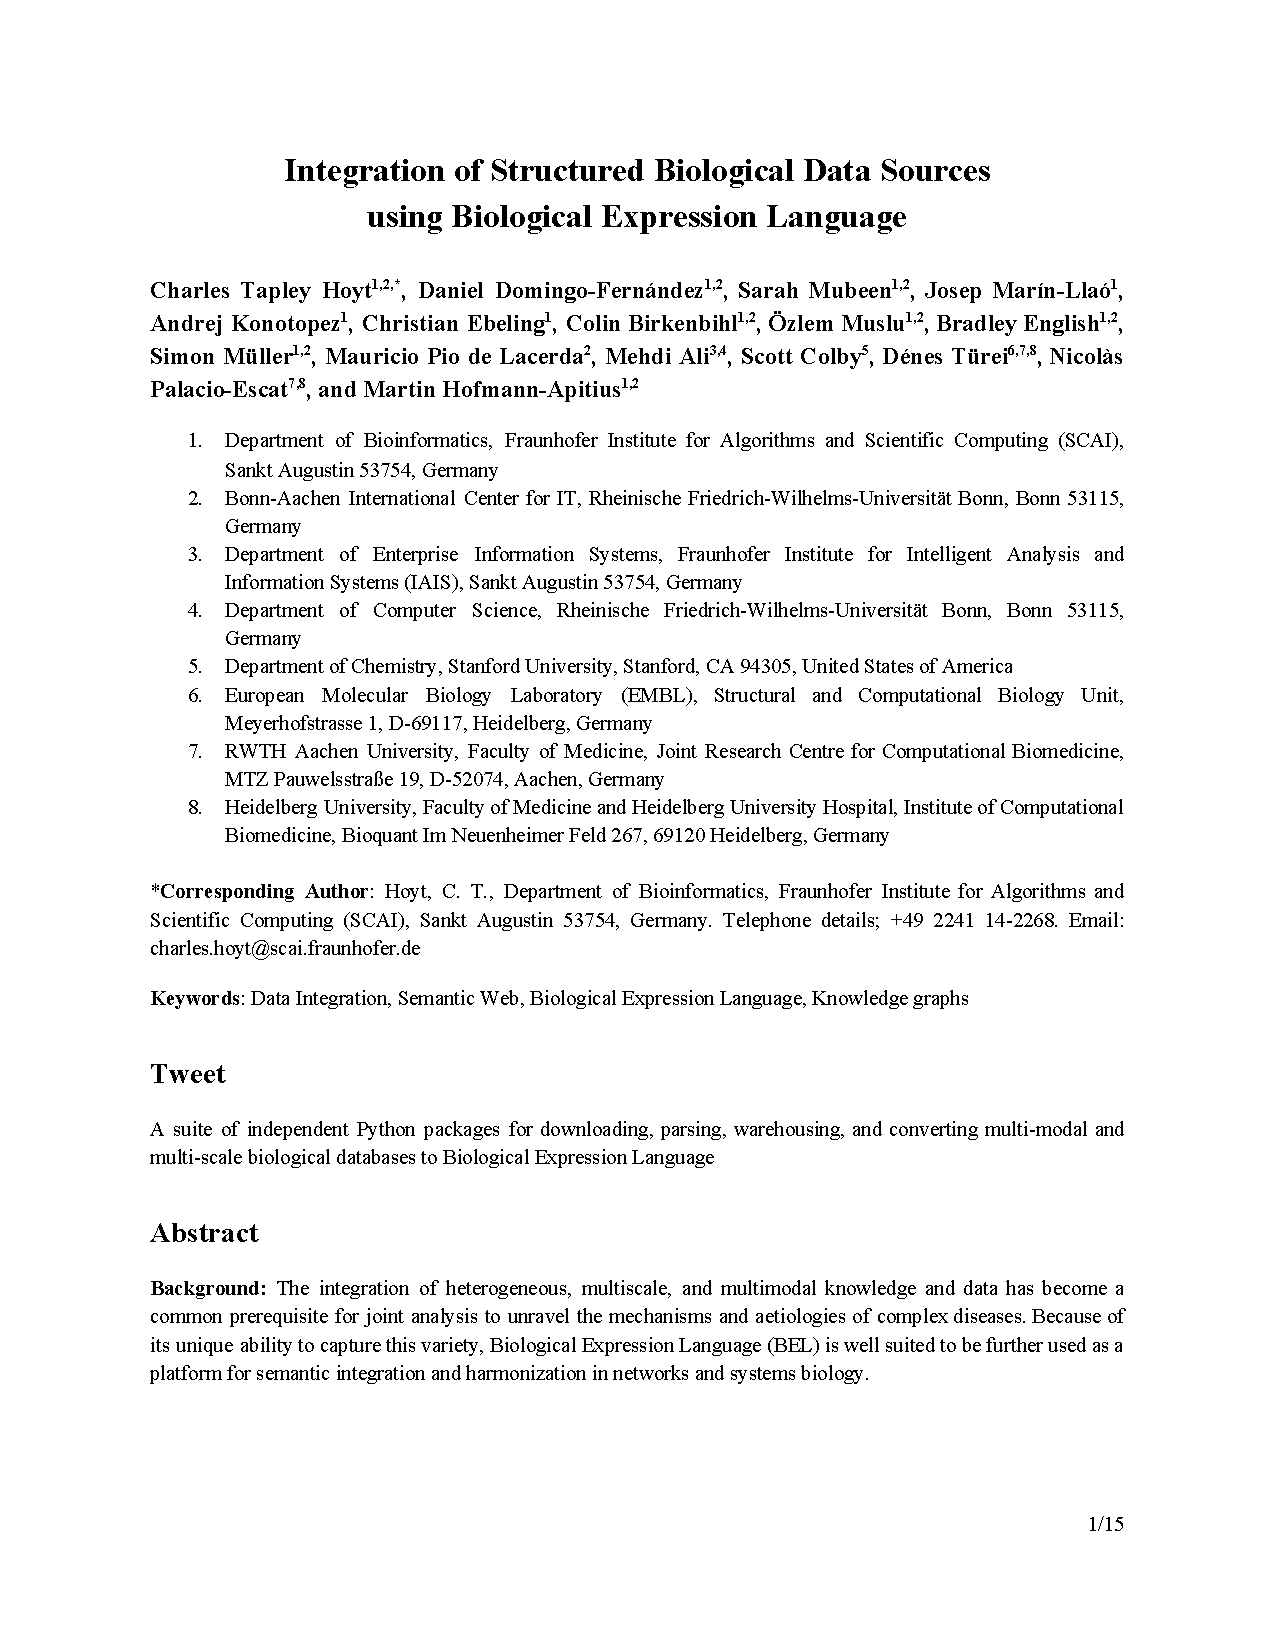
\includepdf[pages={-}]{articles/bio2bel.pdf}

\section*{Postface}

Several applications of Bio2BEL were presented.
First, Bio2BEL enabled the mapping of pathways between databases like \ac{KEGG}~\cite{Kanehisa2017}, Reactome~\cite{Fabregat2016}, and WikiPathways~\cite{Slenter2018} for the ComPath database~\cite{Domingo-Fernandez2018}.
This project leveraged each of these pathway databases as well as nomenclature resources like HGNC, Entrez, UniProt, and ChEBI to normalize entities into cohesive biomedical knowledge graphs on top of which algorithms for identifying overlapping pathways were used to prioritize curation.

Second, the Bio2BEL framework was used to organize the harmonization of pathway databases into a common schema using PathMe~\cite{Domingo-Fernandez2019a}.
This project showcased the Bio2BEL philosophy of reproducibility and reusability because the formats used by each of the pathway databases varied and create significant overhead for new users.

Third, Bio2BEL packages have been used in the application of \ac{NRL} methods using BioKEEN~\cite{Ali2019}.
Because this project saw the generation of a converter for any \ac{BEL} into a format that can be embedded using \ac{NRL}, any new Bio2BEL package can be readily used.

Finally, the Bio2BEL project lead to the integration with several other data aggregation systems.
Integration with \ac{INDRA}~\cite{Gyori2017} was done through the development of the PyBEL processor~\footnote{\url{https://indra.readthedocs.io/en/latest/modules/sources/bel/index.html\#module-indra.sources.bel.processor}} and subsequent inclusion within the Bio2BEL framework\footnote{\url{https://github.com/bio2bel/bio2bel/commit/e52eefad11f38f6654b2c27724ea9f3600f58405}}.
Integration with OmniPath~\cite{Turei2016} was done during the course of the work that comprised the previous publication in the v0.8 release of \textit{PyPath}\footnote{\url{https://github.com/saezlab/pypath}}.
Further systems will be integrated in the future, such as the sources composing Pathway Commons~\cite{Cerami2011}.

Given the PyBEL ecosystem first introduced in Chapter~\ref{ch:pybel}, the environment for exploration presented in Chapter~\ref{ch:belcommons}, the enrichment workflow presented in Chapter~\ref{ch:recuration}, and Bio2BEL, it is possible to generate and handle high quality biological knowledge graphs to support downstream analysis.
The remaining Chapters~\ref{ch:bel2abm},~\ref{ch:guiltytargets}, and~\ref{ch:epicom} constitue three examples of these downstream analyses.
